\section{Introduction}

\subsection{\ac{iot} Security}

The ability of ``things'' to connect and interact with each other over the Internet with minimum human involvement makes Internet of Things a new step in technological progress. Thanks to the widespread use of wireless technology and the emergence of cloud computing, the \ac{iot} is growing at an astronomical pace and is expected to reach ``more than 20 billion internet connected things by 2020'' \cite{Gartner17}. However, while \ac{iot} ecosystem can greatly benefit our life, uncontrollable growth of internet-connected devices leads to increased security and privacy risks. Heterogeneous nature of \ac{iot} systems, which can combine millions of distinctive devices, infrastructures and applications, makes it extremely difficult to develop uniform security standards and policies. This greatly widens the attack surface of \ac{iot} devices and makes them particularly attractive to hackers. 

To discuss cybersecurity of any system, we must understand its architecture. Three-layer model is one of the most commonly used \ac{iot} architecture models. The three comprehensive layers/levels in this model are: perception layer, network layer and application layer \cite{Mendez17,Deogirikar17,Krishna17}. Perception layer is responsible for reliable collection of data from various sensors. Perception layer is often built using \ac{rfid} tags and \acp{usn}, which help identify objects and obtain any necessary environmental information \cite{Devera14,Deng12}. Network layer must provide ubiquitous access and reliably transfer any data collected at perception layer. Network layers primarily use wireless communication standards like ZigBee, BLE, Bluetooth (WPAN) and WiFi (WLAN). Application layer is any information processing system that stores and analyzes the received information to appropriately manage an application or a service \cite{Yang17}. In context of cybersecurity each layer can be viewed as separate attack surface with unique vulnerabilities and exploits. Moreover, the interconnectedness of \ac{iot} devices at each layer means that every insufficiently protected device connected to the network can affect the overall level of safety and sustainability of the whole \ac{iot} system. This paper mainly focuses on the perception layer and physical attacks, as we propose a transduction attack on K-type thermocouple sensors and a possible software-based countermeasure. 

\begin{figure} [h]
    \centering
    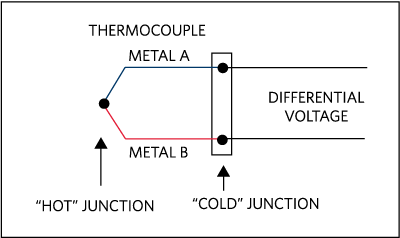
\includegraphics[width=\linewidth]{pictures/TC.png}
    \caption{Fundamental thermocouple \cite{Ismail17}}
    \label{fig:TCouple}
\end{figure}

\subsection{Thermocouple sensors}

Thermocouple is an electric device that utilizes Seebeck effect to measure temperatures at the junction of two dissimilar metals/wires (\cref{fig:Thermocouple}). No power consumption, cost-effectiveness and reasonable accuracy makes K-type thermocouples industry-standard temperature-measuring method \cite{Duff10}. Unfortunately, due to microvolt-level signal changes (~40$\mu$V/\textdegree{}C in K-type), thermocouples are quite susceptible to \ac{emi}/\ac{rfi} \cite{Smalcerz2013,Astm93}. \ac{emi} in this case is any undesirable effects of electromagnetic, electric and magnetic fields, which can degrade the quality of the system due to distortion of the useful signal \cite{Getz96}. This means that without proper physical protection or signal filtering (analog and/or digital) such sensors can be vulnerable to stray noise or a range of intended physical attacks. While proper shielding and dedicated filters can greatly reduce such interference, they can also make an otherwise cheap and robust sensors quite costly and complex. 

\subsubsection{Electromagnetic vulnerabilities}

To test the susceptibility of thermocouple sensors to electromagnetic vulnerabilities, we experimented with one of the possible physical attacks - inducing voltage in the thermocouple wires. Generally, there are two ways in which electromagnetic fields can significantly skew the thermocouple readings: ``induction heating of the thermoelements and induced voltage in the thermocouple wires'' \cite{Omega17}. Heat induction happens at very high amplitudes or high frequencies, when induced currents from alternating magnetic field heat the thermoelement itself, thus affecting the measurement readings. Inducing voltage in thermocouple wires on the other hand, does not require a large field to make any alteration to the temperature output. Since thermocouples measure microvolt-level signal changes, inducing even a small voltage in thermocouple wires can affect the accuracy of the readings. Electromagnetic induction in this case can be explained using Faraday's law of induction \cref{fig:Thermocouple}, which states that ``induced electromotive force (i.e. voltage) in any closed circuit is equal to the rate of change of the magnetic flux enclosed by the circuit'' \cite{Jordan68}. 

\begin{equation}
\begin{split}
\varepsilon = - N\frac{\mathrm{d\Phi _{B}} }{\mathrm{d} t},
\end{split}
\qquad
\begin{split}
\varepsilon \text{- Electromotive force}\\
{\Phi _{B}} \text{- magnetic flux}\\
N \text{- number of coil turns}
\end{split}
\end{equation}

\begin{figure}[h]
    \centering
    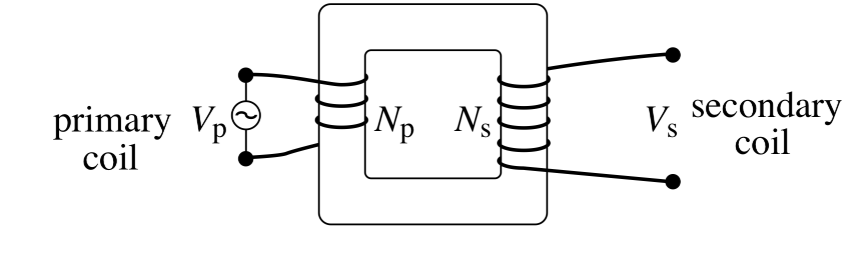
\includegraphics[width=\linewidth]{pictures/FLaw.png}
    \caption{Basic transformer (functions by applying Faraday\textquotesingle s law of induction) \cite{Flap96}}
    \label{fig:Transformer}
\end{figure}


Inducing large voltages can allow the adversary to not only introduce electromagnetic noise to the thermocouple sensors, but completely manipulate the temperature readings. Given a reasonably large amplitude/frequency, the attacker can skew the temperature outputs from thermocouple towards impossibly low or high values [11]. Depending on the final application, incorrect readings from such thermocouple sensors can result in minor inconvenience (home thermostats) or in major accident (flame sensors in gas appliances). 

There are few common solutions to general \ac{emi}/\ac{rfi} problem, like \ac{rfi} filters, differential-input amplifiers, low-pass filters, etc. \cite{Duff10}. However, when the attack is highly directional and operates at high amplitude/frequency, these solutions can make thermocouple systems very expensive and complex. Alternative methods would be software-based countermeasures that focus on anomaly detection algorithms and an appropriate response \cite{Amitai16}. In this paper we propose a software-based countermeasure, which includes a simple guard logic and alert/response algorithm, to help the \ac{iot} sensor systems detect and thwart common transduction attacks.

This paper is organized as follows. In \cref{hwi}, we describe in detail our experiment with one of the transduction attacks on K-type thermocouples. \cref{swi} focuses on our signal filter application, which was implemented in software and can potentially help thwart such attacks. \cref{disc} includes a discussion and analysis of our experiment and simulation results. In \cref{fut}, we look at the possible next steps for this project, such as alternative transduction attacks and some potential improvements to our countermeasure implementation. A brief conclusion is given in \cref{conc}.


